\section{误差}\label{sec:1-3}

\begin{figure}[htbp]
  \centering
  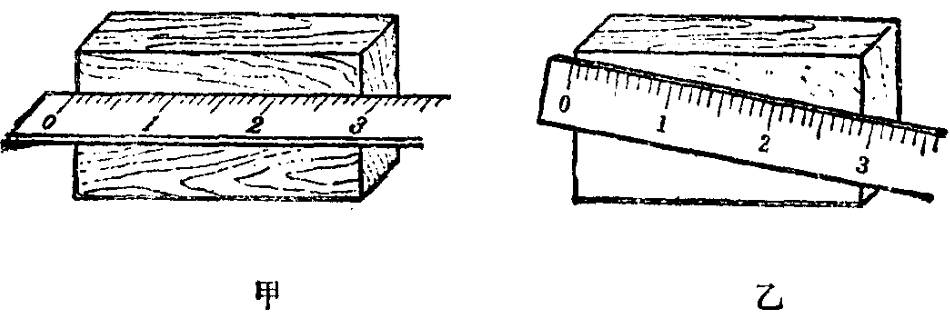
\includegraphics[width=0.6\textwidth]{../pic/czwl1-ch1-11}
  \caption{}\label{fig:1-11}
\end{figure}

测量的时候,如果测量方法不正确,就会产生错误。
使用刻度尺量长度时,必须注意:在用厚刻度尺的时候,尺要照图 \ref{fig:1-11} 甲那样放置,
使刻度贴近被测物体,这样容易看准物体的边线所对的刻度值。
刻度尺在被量物体上的位置不要象图 \ref{fig:1-11} 乙那样歪斜。
观察刻度线的时候,视线要跟尺垂直(图 \ref{fig:1-12})。

\begin{figure}[htbp]
  \centering
  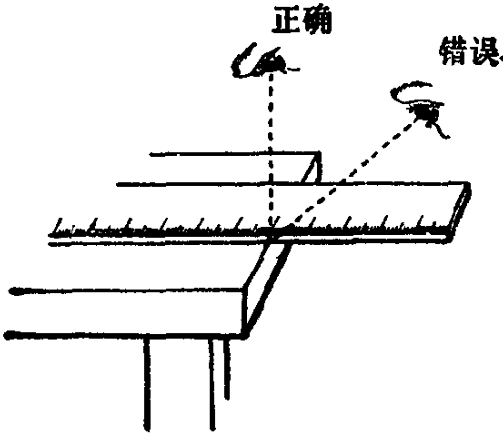
\includegraphics[width=0.4\textwidth]{../pic/czwl1-ch1-12}
  \caption{}\label{fig:1-12}
\end{figure}

两个同学都用正确的测量方法,认真、仔细地测量同一枝铅笔的长度,而测出的结果可能并不完全相同。
但是,一个物体的真实长度总是一定的,我们把物体的真实长度叫做它的真实值。
一般说来,测量值和真实值之间总会有些差异,这个差异叫做\textbf{误差}。
误差和错误不同,错误是应该而且可以避免的,而误差是不能绝对避免的。
误差是怎么产生的呢?

误差的产生跟测量工具有关系。例如刻度尺的刻度不够准确,钢尺的热胀冷缩,还可能有些弯曲,
用它们测长度就会产生误差。测量工具越精密,误差就越小。

误差的产生还跟测量的人有关系。我们知道,用最小刻度是毫米的尺量长度,毫米的下一位数字是估计出来的。
不同的人在估计的时候,有的人估计得偏大些,有的人估计得偏小些。
用秒表测时间的时候,有的人按得早些,有的人按得晚些。
这就产生了跟测量的人有关系的误差。

由于测量时要有估计,所以一个人用同一个测量工具对一个物体测量几次,所得的结果也会不同。
比如一位同学用有毫米刻度的尺先后五次测量一个物体的长度,各次测得的数值分别为

$l_1 = 1.41$ 厘米,$l_2 = 1.42$ 厘米,$l_3 = 1.42$ 厘米,$l_4 = 1.41$ 厘米,$l_5 = 1.43$ 厘米。

各次测得的数值相近,不能说哪一次测量更准确。但是可以想到,有时测量值大于真实值,有时测量值小于真实值,
而多次测量的平均值会更接近真实值,误差较小。因此,我们取五次测量的平均值 $\bar{l}$ 作为测量结果。

$\begin{aligned}[t]
    l &= \dfrac{l_1 + l_2 + l_3 + l_4 + l_5}{5} \\
      &= \dfrac{1.41 \,\text{厘米} + 1.42 \,\text{厘米} + 1.42 \,\text{厘米} + 1.41 \,\text{厘米} + 1.43 \,\text{厘米}}{5} \\
      &= \dfrac{7.09 \,\text{厘米}}{5} = 1.42 \,\text{厘米 。}
\end{aligned}$

误差是不能绝对避免的,但是随着科学技术的发展,精密测量仪器不断出现,
实验方法不断改进,人们减小误差的本领越来越大。
例如,过去用几何方法测量地球到月球的距离,误差有几千米,现在用激光来测,误差就只有几厘米了。

在学习物理的过程中,要做许多实验。做实验的时候,一定要认真、细致,不要出错误。
同时还应该注意分析误差产生的原因,想办法来减小它,提高自己的实验技能。


